\section{ETL}\label{sec:ETL}
The data foundation for this project relies on two sources, refer Section \ref{sec:datafound}. Extract-Transform-Load (ETL) is an important phase for integrating these two sources of information into the data warehouse while ensuring a uniform data-representation. A preprocessing procedure fills static support-tables and dimensions with data. The data available through OpenStreetMap and the INFATI project contains necessities for car information and enough information to start building a GPS Fact. After the preliminary data is loaded into the data warehouse, a number of post-processing procedures fills the remaining tables with data. An overview of the ETL-procedure can be seen in Figure \ref{fig:etl}.

\begin{figure}[tb]
\centering
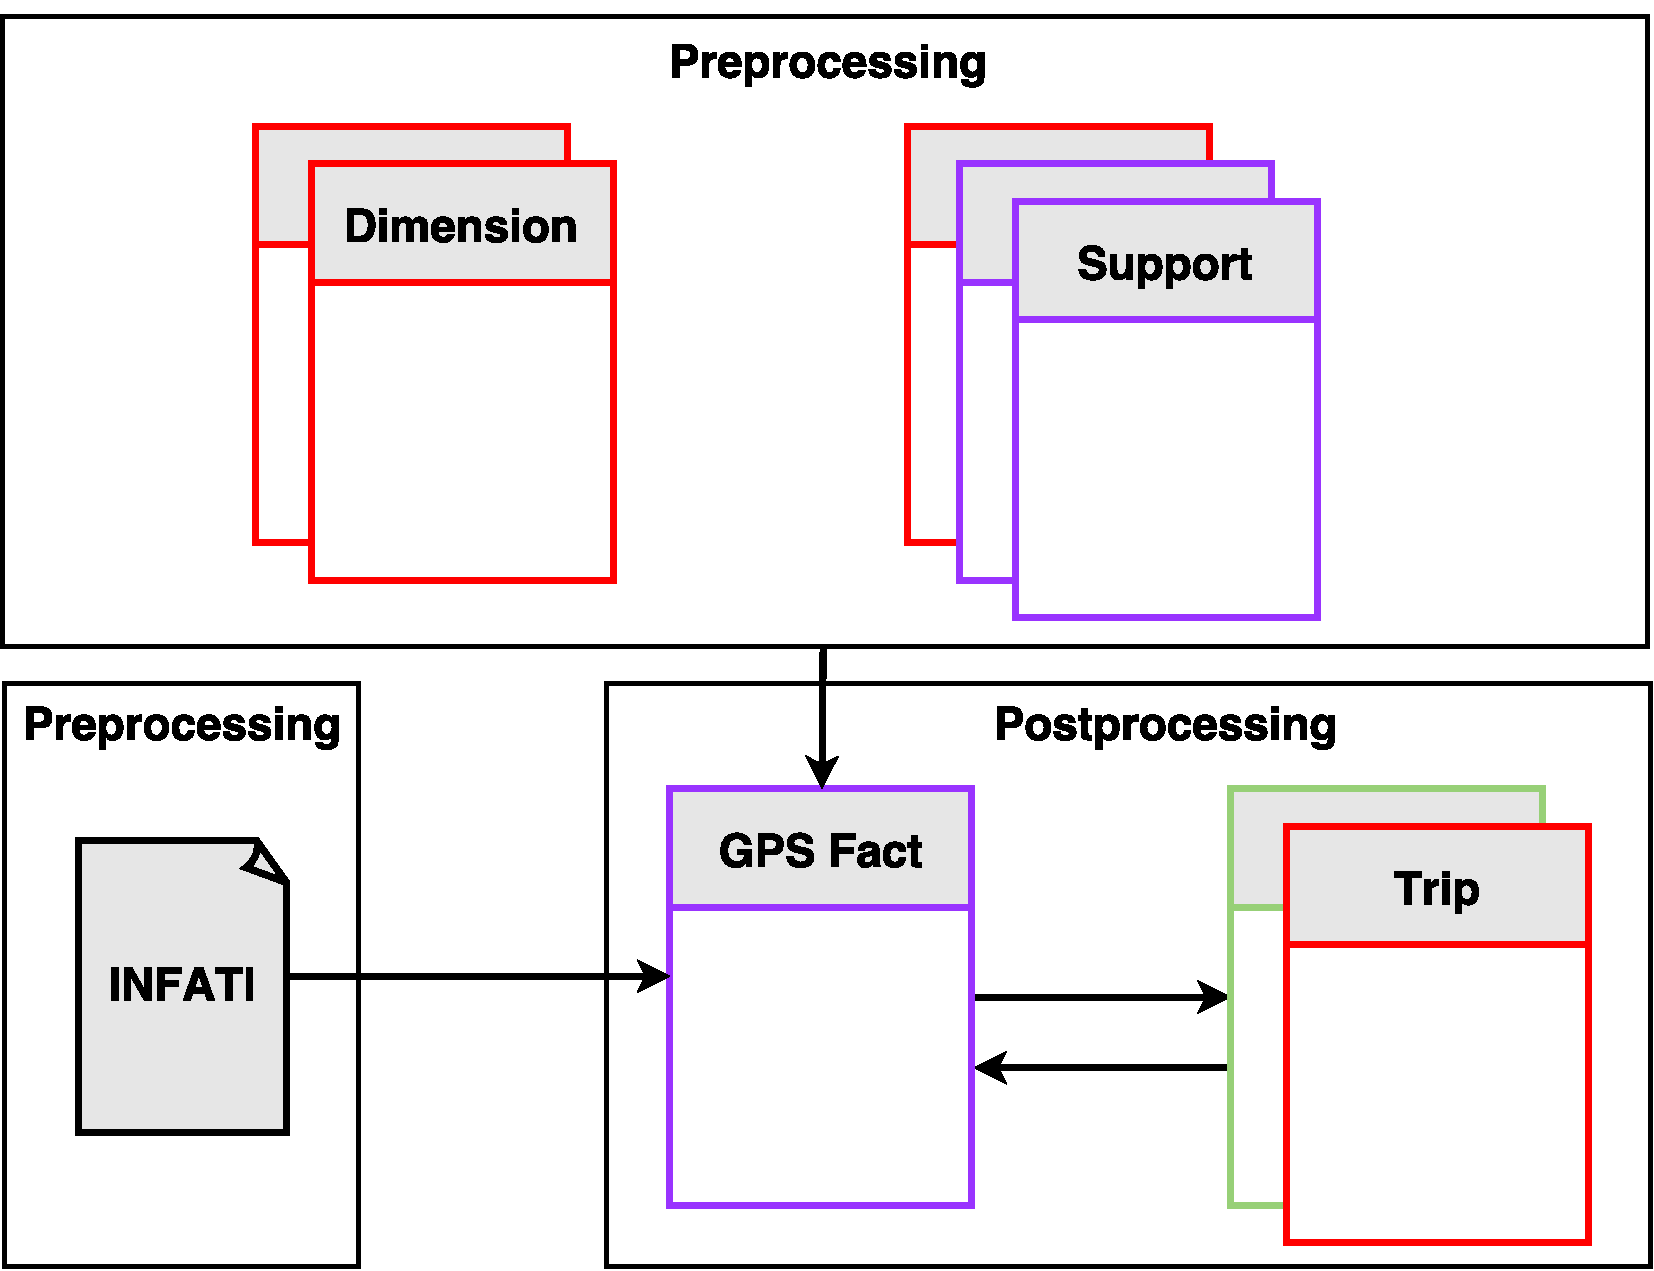
\includegraphics[width=0.465\textwidth]{Pictures/ETL}
\caption{Dataflow throughout the ETL process}
\label{fig:etl}
\end{figure}

The INFATI project\cite{art:INFATI} uses a digital roadmap from OpenStreetMap\cite{osm}. The same digital roadmap is used for this project. A few modifications is introduced, like storing the column \textit{direction} as a smallint instead of a textual representation. 

The INFATI dataset\cite{art:INFATI} contains 17 columns of data, separated by a varying number of spaces. Due to the natural challenges of map-matching, some entries have not been map-matched successfully. These rows contain only 14 columns of data. This renders the dataset unreadable, due to problems with trailing zeros, when loading with a space-separator. To ease the ETL process, a script was made to change and fix the separator. In this script \# is used as delimiter, and whenever a row was not map-matched, three \#'s are appended to that row.

INFATI coordinate-sets are stored in the geodetic datum ED50, within UTM zone 32N. The system proposed in this paper is built on GPS, and a transformation from UTM to lattitude and longitude is needed. Coordinate-sets are stored as points, lines or polygons and stored in the data warehouse as PostGIS\cite{postgis} geometries. These geometries has to be assigned the correct spatial reference system identifier(SRID), in order to display a position correctly. With the INFATI dataset being logged in ED50 and UTM zone 32N, this corresponds to a SRID of 23032\cite{UTM32N}. Latitude and longitude format is part of World Geodetic System(WGS), latest edition being WGS84 and has SRID 4326\cite{WGS84}. To transform the INFATI data into the desired format the geometry is created, assigned the appropriate SRID of 23032, and then transformed into latitude and longitude format using the SRID of 4326.

The last part of preprocessing is adding the appropriate data for the support-table \textit{Quality Information} and the dimensions \textit{Date} and \textit{Time} are computed and stored. For \textit{Quality Information} this means storing each combination of HDOP and satellites. This completes the filling of the static support tables.

Before loading the GPS data from the INFATI data-set, a car must be created and stored in \textit{Car Information}. The corresponding INFATI data then has to be loaded into \textit{GPS Fact}. 

Three postprocessing-steps will now fill in missing measures.

The first step is dividing the batch of gpsfacts into trips for each car and each trip will be stored in an empty tripfact, with a TripId. That tripfact will then be assigned the appropriate CarId, and the gpsfacts belonging to that trip will be updated with the assigned TripId. This is done by fetching the gpsfact from the data warehouse, and sort them based on their timestamp. A new instance of a trip is created, and gpsfacts are continuously stored into this trip. When a timestamp is more than three minutes older than the previous, a new trip is instantiated. The process continues till the point where all gpsfacts are contained a trip. This makes it possible to  assign a correct TripId to each gpsfact.

The second step is calculating all the missing measures for all gpsfacts. The process will take one car at a time, fetch all TripIds for that car, go through one trip at a time. It will fetch the gpsfacts for that trip, calculate the measures, and update each gpsfact accordingly. This is done by fetching all gpsfacts for a certain trip, and sort them based on their timestamp. A loop will then start working from the 2nd entry, and calculate measures based on what happened since the previous entry.  By example, the acceleration metric is calculated by taking the change in speed from a given gps-point to a previous point, and divide it with the time difference from previous point. These metrics will be saved given gpsfact. Once a trip runs out of gpsfacts, these gpsfacts will be updated in the data warehouse.

The third step begins when the \textit{GPS Fact} has been updated with measures, because it is possible to compute the measures for each tripfact. The process will take one car at a time, fetch all TripIds for that car, go by one trip at a time, fetch all gpsfacts for that trip, use gpsfacts to compute measure, and update the tripfact with these measures. This is done by looping over all gpsfacts, counting total amounts of contingencies for the different metrics. The intervals is then filled with the appropriate percentages, relative to the total counts, based on the distribution of the severity of the contingencies. Additionally, the trivial measures like when the trip started, total meters driven, etc. are aggravated. When all the measures are calculated, the tripfact is updated in the data warehouse.

\textit{SubTrip Fact} is only conceptual at this time. Nothing is calculated or stored in the data warehouse. Given the similarities between \textit{SubTrip Fact} and \textit{SubTrip Fact}, it would however use many of the same computations as \textit{TripFact} which would make this process relatively trivial.

If a data source other than INFATI were to be used in the future, some of the ETL procedure would have to be redesigned, as some of the implementation is written specifically to handle the INFATI data. As such we would need another process for transforming the data into the uniform data-representation present in the data warehouse.

%Måske skal det her ikke med?
%To decrease the computation-time of the ETL-phase, the loading-process has been multi-threaded so that a single car is being loaded in its individual thread. This is only relevant for the INFATI dataset. In a working setting, data would come in bulks of single trips. 
